% DO NOT COMPILE THIS FILE DIRECTLY!
% This is included by the other .tex files.

\begin{frame}[t,plain]
\titlepage
\end{frame}

\begin{frame}
    \frametitle{Outline of the presentation}
    \begin{itemize}
        \item Present the features available for Sharing \textit{galaxy clusters}
        \item Look at the internals of what changed in the datamodel and MISP's behaviors
    \end{itemize}
\end{frame}

\begin{frame}
    \frametitle{MISP Galaxy 2.0}
    Galaxy 2.0 introduces various new features for \textit{Galaxies} and their \textit{Clusters} allowing:
    \begin{itemize}
        \item Creation of \textbf{custom} \textit{Clusters}
        \item \textbf{ACL} on \textit{Clusters}
        \item \textbf{Connection} of \textit{Clusters} via \textit{Relations}
        \item \textbf{Synchronization} to connected instances.
        \item \textbf{Visualization} of forks and relationships
    \end{itemize}
\end{frame}

\begin{frame}
    \frametitle{Default Galaxy clusters}
    {\bf Default} {\it Galaxy cluster} 
    \begin{itemize}
        \item Coming from the \texttt{misp-galaxy} repository\footnote{\url{https://github.com/MISP/misp-galaxy}}
        \item Cannot be edited
        \begin{itemize}
            \item Only way to provide modification is to modify the stored JSON or to open a pull request
            \item Are not synchronized
            \item Source of trust
        \end{itemize}
        \item Restrictions propagate to their children (\texttt{Galaxy cluster elements}, \texttt{Cluster relationships})
    \end{itemize}

    \vspace{0.5em}
    {\bf Custom} {\it Galaxy cluster} 
    \begin{itemize}
        \item Can be created via the UI or API
        \item Belongs to an organisation
        \begin{itemize}
            \item Fully editable
            \item Are synchronized
        \end{itemize}
    \end{itemize}
\end{frame}


\begin{frame}
    \frametitle{MISP Galaxy 2.0 - Comparison with prior version}
    \textit{Clusters} and \textit{Relations} can be edited.
    \begin{itemize}
        \item New \textit{Clusters} fields
        \begin{itemize}
            \item \texttt{distribution}, \texttt{sharing\_group\_id}
            \item \texttt{org\_id}, \texttt{orgc\_id}
            \item \texttt{locked}, \texttt{published}, \texttt{deleted}
            \item \texttt{default}
            \begin{itemize}
                \item \textit{Clusters} coming from the \texttt{misp-galaxies} repository are marked as default
                \item Not synchronized
            \end{itemize}
            \begin{itemize}
                \item Same purpose as \textit{Event}'s \texttt{locked} field
            \end{itemize}
            \item \texttt{extends\_uuid}
            \begin{itemize}
                \item Point to the \textit{Cluster} that has been forked
            \end{itemize}
            \item \texttt{extends\_version}
            \begin{itemize}
                \item Keep track of the \textit{Cluster} version that has been forked
            \end{itemize}
        \end{itemize}
    \end{itemize}
\end{frame}

\begin{frame}
    \frametitle{MISP Galaxy 2.0 - Others changes}
    \begin{itemize}
        \item \textit{Role} \texttt{perm\_galaxy\_editor}
        \item Relations also have a \texttt{distribution} and can have \textit{Tags}
        \item Synchronization servers have 2 new flags
        \begin{itemize}
            \item \texttt{pull\_galaxy\_clusters}
            \item \texttt{push\_galaxy\_clusters}
        \end{itemize}
        \item Clusters \texttt{blocklist}
    \end{itemize}
\end{frame}

\begin{frame}
    \frametitle{Features in depth: CRUD}
    \begin{itemize}
        \item Standard CRUD
        \item Soft and Hard deletion
        \item Publishing
        \item Update forked cluster to keep it synchronized with its parent
        \item ACL on the \textit{Cluster} itself, not on its tag
        \begin{itemize}
            \item \texttt{misp-galaxy:{\color{blue} galaxy-type}="{\color{red} cluster UUID}"}
            \item \texttt{\tiny misp-galaxy:{\color{blue} mitre-attack-pattern}="{\color{red} e4932f21-4867-4de6-849a-1b11e48e2682}"}
        \end{itemize}
    \end{itemize}
\end{frame}

\begin{frame}
    \frametitle{Features in depth: Visualization}
    Tree view of forked Clusters
    
\includegraphics[scale=0.5]{pics/cluster-forks}
    \vspace{0.5em}
    \begin{center}
        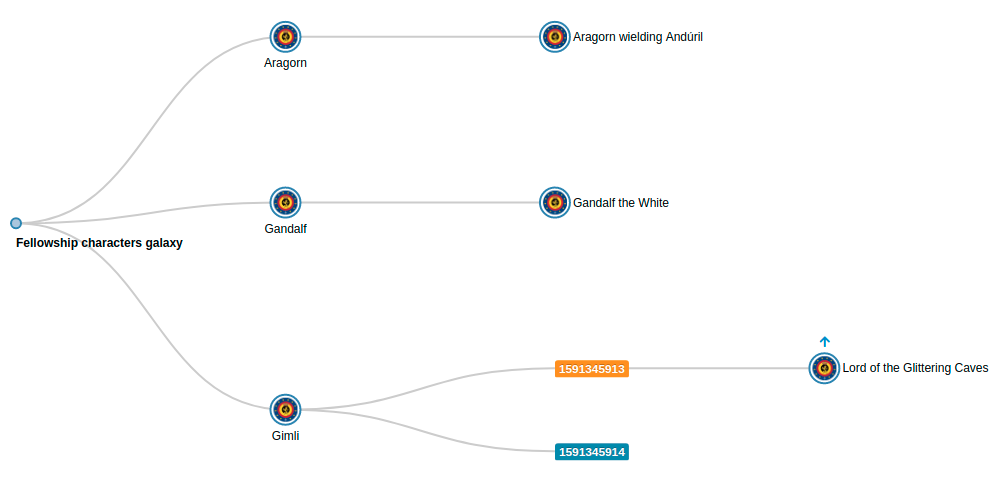
\includegraphics[width=1.0\linewidth]{pics/cluster-forks-tree}
    \end{center}
\end{frame}

\begin{frame}
    \frametitle{Features in depth: Visualization}
    Tree and network views for Relations between Clusters
    \vspace{0.5em}
    \begin{center}
        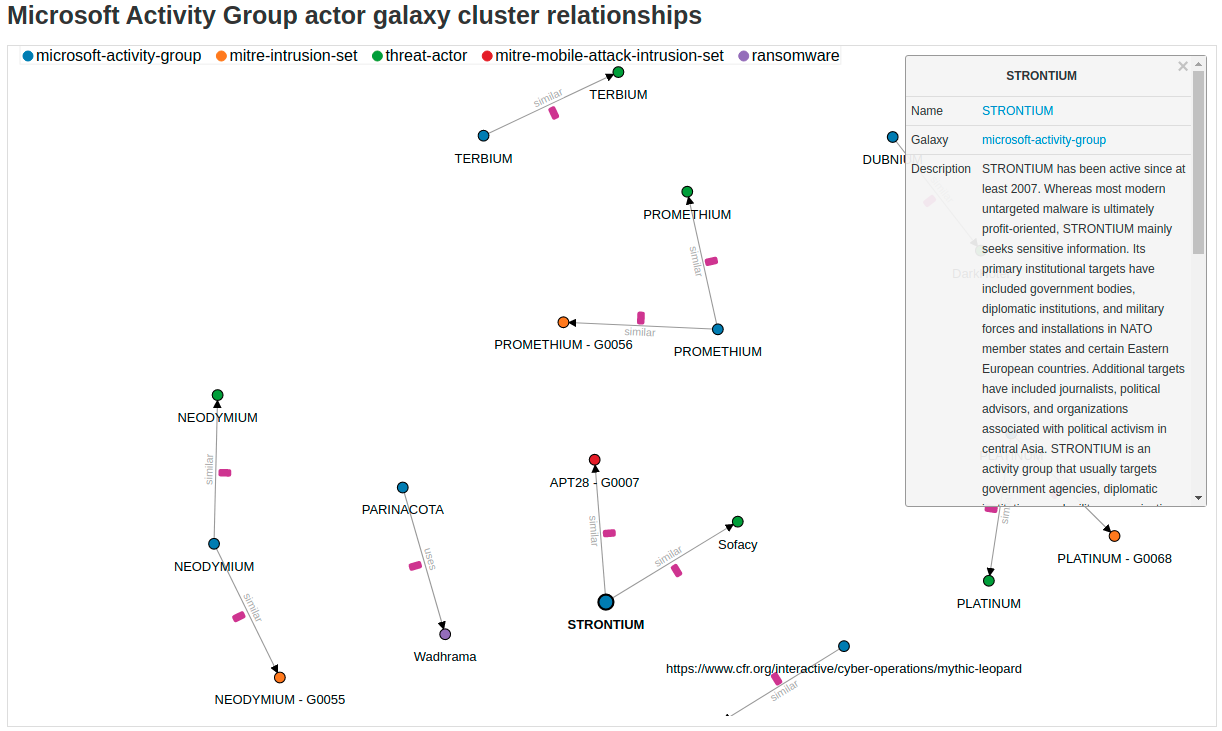
\includegraphics[width=1.0\linewidth]{pics/cluster-relations}
    \end{center}
\end{frame}

\begin{frame}
    \frametitle{Features in depth: Visualization}
    Tree and network views for Relations between Clusters
    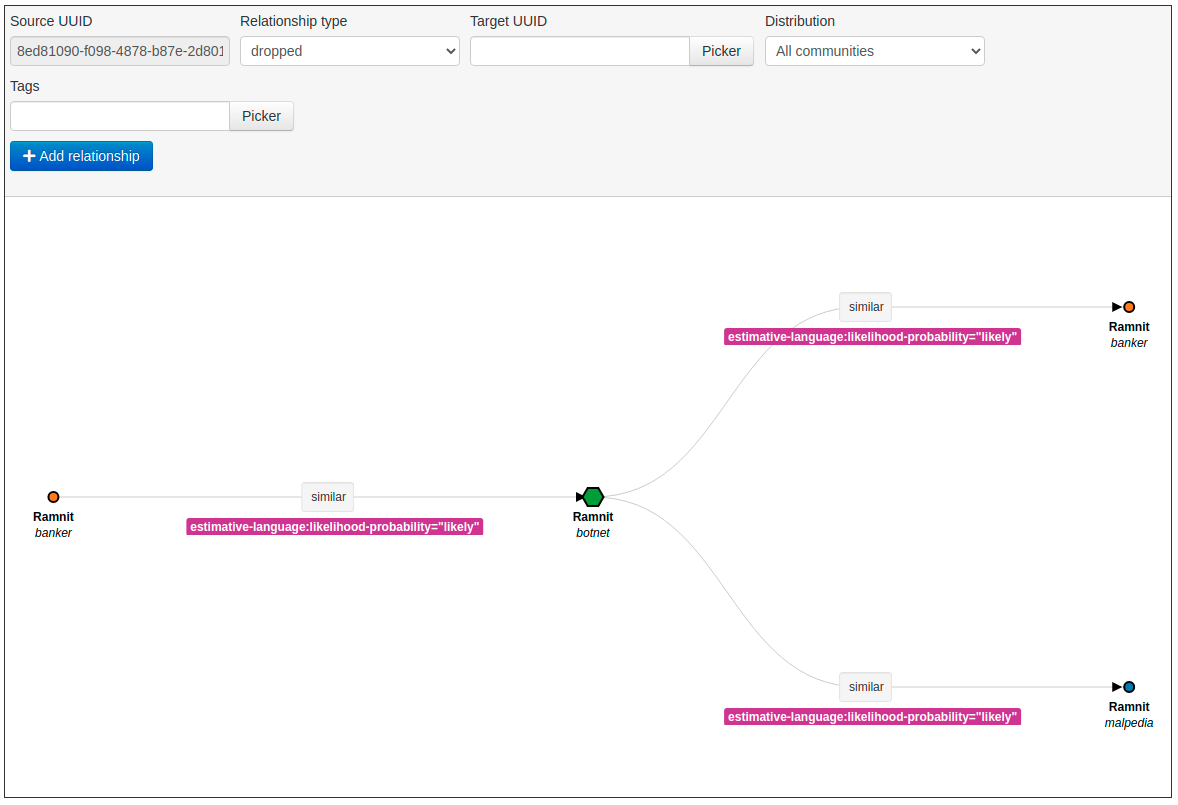
\includegraphics[width=1.0\linewidth]{pics/cluster-relations-tree}
\end{frame}

\begin{frame}
    \frametitle{Galaxy cluster elements}
    Hasn't been touched: Still a key-value stored. But new feature have been added\footnote{Will be included in next release}
    \vspace{0.5em}

    Tabular view
    \begin{itemize}
        \item Allows you to browse {\bf cluster elements} like before
    \end{itemize}
    \begin{center}
        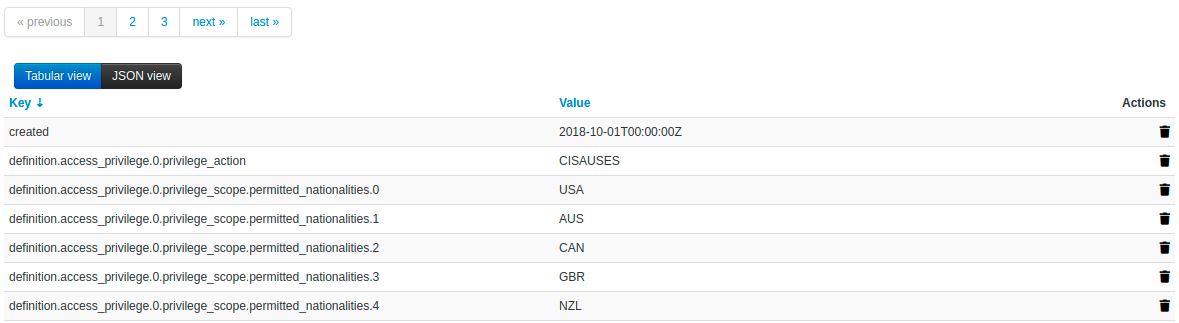
\includegraphics[width=1.0\linewidth]{pics/tabular-view.png}
    \end{center}
\end{frame}

\begin{frame}
    \frametitle{Galaxy cluster elements}
    JSON view
    \begin{itemize}
        \item Allows you to visualisation {\bf cluster element} in a JSON structure
        \item Allows you to convert any JSON into {\bf cluster elements} enabling searches and correlations
    \end{itemize}
    \begin{center}
        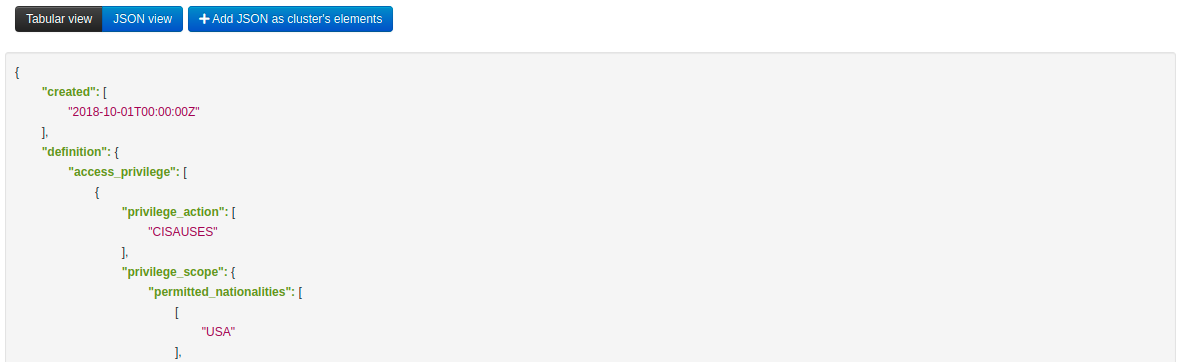
\includegraphics[width=1.0\linewidth]{pics/json-view.png}
    \end{center}
\end{frame}

\begin{frame}
    \frametitle{Synchronization in depth}
    Has its own synchronization mechanism which can be enabled with the \texttt{pull\_galaxy\_cluster} and \texttt{push\_galaxy\_cluster} flags
    \vspace{0.5em}
    \begin{itemize}
        \item \textbf{Pull All}: Pull all remote Clusters (similar to event's pull all)
        \item \textbf{Pull Update}: Update local Clusters (similar to event's pull update)
        \item \textbf{Pull Relevant}: Pull missing Clusters based on local Tags
        \item \textbf{Push}: Triggered whenever a Cluster is published or via standard push
    \end{itemize}
\end{frame}
